%\documentclass[linenumbers, RNAAS, trackchanges]{aastex631}
\documentclass[linenumbers, twocolumn]{aastex631}

\usepackage[utf8]{inputenc}
\usepackage{hyperref}           % hrefs
\usepackage{natbib}             % for bibliography
\usepackage{float}              % figure positioning
\usepackage{svg}                % used for SVG images
\usepackage{graphicx}           % used for non-SVG images
\usepackage{amsmath}
\usepackage{parskip}


% Search Query Metadata
\shorttitle{Bessel Functions}
%\shortauthors{Nguyen & Sae}

% Hyperlink setup
\hypersetup{
colorlinks=true,
linkcolor=blue,
urlcolor=blue
}

\begin{document}
\title{Numerical Analysis of Bessel Function Roots and Applications in Physical Systems}
% [] is for ORCiD
%\correspondingauthor{Main Author}
%\email{author1@email.com, author2@email.com, author3@email.com}
\author{Lily Nguyen}
\affiliation{Department of Physics, The University of Texas at Austin\\
Austin, TX 78712, USA}

\author{Andre Sae}
\affiliation{Department of Physics, The University of Texas at Austin\\
Austin, TX 78712, USA}


% 250 word limit for abstract
\begin{abstract}

We numerically computed and visualized the first five positive
roots of the Bessel functions of the first kind, $J_0(x)$, $J_1(x)$, and $J_2(x)$,
using Python. These functions solve a second-order differential equation that 
occur in problems with radial symmetry. We used the \texttt{scipy} library to
evaluate $J_n(x)$ and locate its roots via the \texttt{fsolve} method. We
interpreted the computed roots in the context of three physical materials: the
radial wavefunction in a quantum infinite square well, heat conduction in
cylindrical geometries, and vibrational modes of a circular drumhead. Our
results show how Bessel function roots reflect physical boundary conditions
and highlight the usefulness of numerical methods in modeling such systems.

\end{abstract}

% Use astrothesaurus numbers in place of num
\keywords{Bessel functions --- root-finding --- radial symmetry --- boundary conditions --- numerical analysis}


\section{Introduction} \label{sec:intro}

The Bessel functions of the first kind, $J_n(x)$, are solutions to the
second-order linear differential equation:
\begin{equation}
    z^2\frac{d^2 w}{dz^2}+z\frac{dw}{dz}+(z^2-n^2)w=0,
\end{equation}
\noindent where integer $n=0,1,2\dots$ represents the order of the
function. These functions appear in the separation of variables when solving
partial differential equations in cylindrical or spherical coordinates,
particularly in systems with radial symmetry \cite{abramowitz_stegun}. Bessel functions also have an
integral
\begin{equation}
    J_n(x)=\frac{1}{\pi}\int_0^\pi cos(x\sin\theta-n\theta)d\theta
\end{equation}
\noindent for integers $n=0,1,2\dots$, which is useful for understanding 
their oscillatory behavior.

\noindent Bessel functions were first introduced by German astoronomer and
mathematician Friedrich Wilhelm Bessel in the early 1800s during his study of
planetary orbits. However, the equation itself had been investigated earlier
by Bernoulli and Euler in problems involving vibrational membranes
\citet{abramowitz_stegun}. Today, Bessel functions are foundational tools in 
mathematical physics and engineering. In quantum mechanics, they appear in 
radial solutions to the Schrödinger equation for quantum wells \cite{hanson}, in the 
vibration modes of circular membranes like drumheads \cite{tamrin}, and in heat 
conduction problems with cylindrical geometries \cite{neils}.

\noindent In this project, we numerically compute the first five positive roots
of the Bessel functions $J_0(x)$, $J_1(x)$, and $J_2(x)$. These roots correspond
to physically meaningful quantities such as resonance modes, cutoff frequencies, 
or quantized boundary values in systems with radial symmetry. We use Python to visualize each
function, estimate the approximate locations of their roots, and apply the \texttt{fsolve}
method from \texttt{scipy.optimize} to compute each root. 
Our goal is to obtain accurate root values for each order
using numerical methods.\\


\section{Data and Observations} \label{sec:data}

This project focuses on computing and visualizing the first five roots of the
Bessel functions of the first kind, $J_n(x)$, for orders $n=0,1,2$. These
functions solve the second-order linear differential equation:
\begin{equation}
    z^2\frac{d^2 w}{dz^2}+z\frac{dw}{dz}+(z^2-n^2)w=0,
\end{equation}
\noindent which appear in physical systems with radial 
symmetry \citet{abramowitz_stegun}. The positive roots of $J_n(x)$ represent physically meaningful
quantities such as resonant frequencies or quantized energy levels in such
systems.

\noindent We computed the Bessel functions using Python's \texttt{scipy.special.jv}
method, which evaluates $J_n(x)$ for an arbitrary order and argument. To
find the roots numerically, we used the \texttt{fsolve} method from \texttt{scipy.optimize},
which refines an initial guess until it finds a point where the function crosses
zero. We chose a set of initial guesses based on where the function appeared to
cross the x-axis in the plot and passed those values into \texttt{fsolve} to
calculate each root more precisely. 

\noindent We used the following initial guesses:
\begin{itemize}
    \item $J_0(x)$: [2, 6.1, 8.6, 11.7, 15]
    \item $J_1(x)$: [3.9, 7, 10.15, 13.1, 16.4]
    \item $J_2(x)$: [5.1, 8.3, 11.8, 14.9, 18]
\end{itemize}

\noindent This gave us exactly five positive roots for each Bessel function. The 
resulting plots of $J_0(x)$, $J_1(x)$, and $J_2(x)$ over the domain $x=0$ to
$x=20$ are shown in Figure~\ref{fig:bessel_roots}, with the first five roots of
each function marked as scatter points.

\begin{figure}[H]
    \centering
    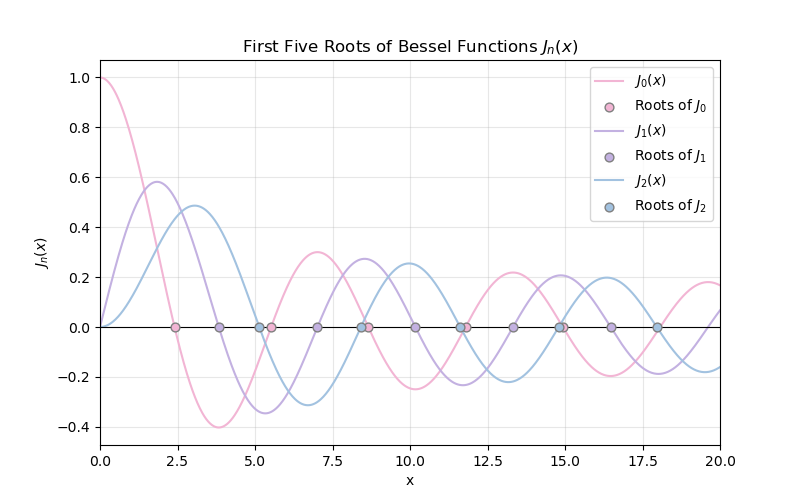
\includegraphics[width=1.0\linewidth]{bessel_roots.png}
    \caption{Bessel functions $J_0(x)$, $J_1(x)$, and $J_2(x)$ plotted from $x=0$ to
    $x=20$, with their first five positive roots represented as circular markers.}
    \label{fig:bessel_roots}
\end{figure}


\section{Results} \label{sec:results}

The plots of $J_0(x)$, $J_1(x)$, and $J_2(x)$ from $x=0$ to $x=20$ show that
Bessel functions of the first kind exhibit oscillatory behavior with a gradually
decaying amplitude. As expected, $J_0(x)$ begins at $1$, while higher-order
functions satisfy $J_n(x)=0$. The zero crossings become slightly less
frequent as $x$ increases.

\noindent The computed roots correspond to the first five positive values of $x$
for which $J_n(x)=0$ and are marked as circular points in Figure~\ref{fig:bessel_roots}.
These roots are important in radial problems where boundary conditions require the
function to vanish at a specific radius. For example, they determine the allowed
energy levels in circular quantum wells, resonance frequencies in drumhead 
vibrations, and decay rates of thermal modes in cylindrical heat conduction.

\noindent Our numerical results followed the expected trend that root values
increase with both the order $n$ and the root index. The quantized structure
highlights the physical significance of Bessel function solutions in bounded
radial domains.\\


\section{Applications} \label{sec:applications}

Bessel functions appear in the solutions of physical
problems that exhibit radial symmetry. In this section, we highlight three
examples: the infinite square well in quantum mechanics, radial thermal
diffusion, and wave propagation on a circular membrane. In each case, Bessel
functions emerge from imposing boundary conditions on the radial part of a 
separable partial differential equation.\\

\subsection{Quantum Mechanics: The Infinite Square Well}

Bessel functions appear in the solution to the Schrödinger equation for a
particle confined in a three-dimensional infinite spherical potential well.
The potential is defined as:
\begin{equation}
    V(x)=
    \begin{cases}
        0, &\text{if }r < a\\
        \infty, &\text{if }r\geq a
    \end{cases}
\end{equation}
\noindent Inside the well ($r < a$), the time-independent Schrödinger equation in
spherical coordinates becomes:
\begin{equation}
    \hat{H}\psi-E\psi=\hat{H}R_{n,l}-ER_{n,l}=0
\end{equation}
\begin{equation}
    \hat{H}=\frac{-\hbar ^2}{2m}\left(\frac{\partial^2}{\partial r^2} + \frac{2}{r} \frac{\partial}{\partial r} - \frac{l(l+1)}{r^2}\right) +V(r)
\end{equation}
\noindent where $R_{n,l}(r)$ is the radial wavefunction, $n$ is the principle
quantum number, $l$ is the angular momentum quantum number, $m$ is the
particle mass, and $\hbar$ is the reduced Planck constant \citet{hanson}.

\noindent With $V(r)=0$ inside the well, the radial differential equation
reduces to:
\begin{equation}
    r^2\frac{\partial^2 R_{n,l}}{\partial r^2} + 2r\frac{\partial R_{n,l}}{\partial r} +(k^2r^2-l(l+1))R_{n,l}=0
\end{equation}
\noindent This is the spherical Bessel differential equation where its solutions
are spherical Bessel functions $j_l(k_{n,l}r)$ These relate to the ordinary
Bessel functions by:
\begin{equation}
    j_l(k_{n,l}r)=\sqrt{\frac{\pi}{2kr}}J_{l+\frac{1}{2}}(k_{n,l}r)
\end{equation}
\noindent To satisfy the boundary condition that the wavefunction vanishes at
$r=a$, we require that $j_l(k_{n,l}a)=0$. This quantization conditions selects
discrete values $k_{n,l}$, which in turn determine the allowed energy levels:
\begin{equation}
    E_{n,l}=\frac{\hbar^2k_{n,l}^2}{2ma^2}
\end{equation}
\noindent The roots of the spherical Bessel functions determine the
quantized energy spectrum of the particle in the well, which illustrates how
the mathematical properties of Bessel functions have direct physical 
consequences in radially symmetric quantum systems \cite{weisstein}.\\


\subsection{Thermal Diffusion}

Bessel functions also appear in heat conduction problems with radial symmetry.
In a two-dimensional circular region, the temperature distribution $T(r,t)$
evolves according to the heat equation:
\begin{align}
    \frac{\partial T}{\partial t}&=\alpha\nabla^2T\\
    &=\alpha\left(\frac{1}{r} \frac{\partial T}{\partial r} + \frac{\partial^2 T}{\partial r^2}\right)
\end{align}
\noindent where  $\alpha=\frac{k}{\rho c_p}$ is the thermal diffusivity, with
$k$ as the thermal conductivity, $\rho$ the material density, and $c_p$ the
specific heat capacity \cite{hahn}.

\noindent To solve this equation, we assume separable solutions of the form
$T(r,t)=X(r)\theta(t)$, which leads us to two ordinary differential equations.
The time-dependent part gives exponential decay:
\begin{equation}
    \frac{d\theta}{dt}+\lambda^2\alpha\theta=0
\end{equation}
\noindent and the spatial part gives the Bessel differential equation
of order zero:
\begin{equation}
    \frac{d^2X}{dr^2}+\frac{1}{r}\frac{dX}{dr}+\lambda^2X=0
\end{equation}
\noindent The general solution involves $J_0(\lambda r)$, and applying boundary
conditions quantizes the solutions in terms of the roots $\beta_n$ where
$J_0(\beta_n)=0$ \cite{tsega}.

\noindent We impose the initial condition $T(r,0)=T_2$ and the boundary condition
$T(R,t)=0$, where $R$ is the radius of the domain and $T_1,T_2$ are constant
values. The resulting dimensionless solution can be written as:
\begin{equation}
    T^*(r,t)=\frac{T(r,t)-T(R,t)}{T(r,0)-T(R,t)}=2\sum_{n=0}^\infty e^{-\beta_n^2\frac{\alpha t}{R^2}}\frac{J_0(\beta_n\frac{r}{R})}{\beta_nJ_1(\beta_n)}
\end{equation}
\noindent which makes the full temperature solution:
\begin{equation}
    T(r,t)=T^*(T(r,0)-T(R,t))+T(R,t)
\end{equation}
\noindent The temperature function uses both the zeroth and first order
Bessel function in the solution, and each mode decays exponentially at a rate set 
by $\beta_n$. Therefore, we see how the Bessel function determines the 
dynamics of thermal modes \cite{neils}.\\


\subsection{Drum Wave Propagation}

The vibration of a circular membrane, such as a drumhead, is another example of
where Bessel functions appear. The vertical displacement of the membrane, $z(r,\theta,t)$,
satisfies the two-dimensional wave equation:
\begin{equation}
    \frac{\partial^2z}{\partial t^2}=c^2\nabla^2z
\end{equation}
\noindent where $c=\sqrt{\frac{S}{\sigma}}$ is the wave speed, $S$ is the surface
tension, and $\sigma$ is the surface mass density of the membrane. 

\noindent Assuming symmetry about the axis (no $\theta$-dependence) and using
separation of variables with $z(r,\theta,t)=R(r)T(t)\Theta(\theta)=R(r)T(t)$,
we obtain two ordinary differential equations. The time-dependent part gives:
\begin{equation}
    \frac{d^2T}{dt^2}+\lambda^2c^2T=0
\end{equation}
\noindent which describes simple harmonic motion in time, and the radial part
 becomes the Bessel differential equation of order $n$:
\begin{equation}
    r^2\frac{\partial^2R}{\partial r^2}+r\frac{\partial R}{\partial r}+(\lambda^2r^2-n^2)R=0.
\end{equation}
\noindent with solutions $R(r)=J_m(\lambda r)$. $J_m$ is the Bessel
function of the first kind.

\noindent When we impose the boundary condition that the membrane is fixed at
its edge ($z(R_f,t)=0$), we can quantize the allowable modes. $\lambda$
must be one of the roots $\lambda_{m,k}$ of the Bessel 
function $J_m(\lambda r)$, which satisfies:
\begin{equation}
    J_m(\lambda_{m,k}R_f)=0.
\end{equation}
\noindent We can write the general solution as a double sum over all radial and
angular modes:
\begin{equation}
    z(r,t)=\sum_{m=0}^\infty \sum_{k=1}^\infty J_m(\lambda_{m,k}r)e^{-c\lambda_{m,n}t}
\end{equation}
\noindent These quantized roots $\lambda_{m,k}$ determine the resonant frequencies
of the membrane. Each pair of integers ($m,k$) corresponds to a distinct
vibration mode, where $m$ is the order of the Bessel function and $k$ is the wavenumber.
For $m=0$, the Bessel function vanishes at the boundary. The final waveform
$z(r,t)$ describes the motion of the drumhead as a superposition of these modes evolving in time \cite{tamrin}.\\


\section{Summary and Conclusion} \label{sec:summary}

We explored the roots of Bessel functions of the first kind, 
$J_n(x)$, for orders $n=0,1,2$ using Python's \texttt{scipy} library. Our numerical
approach combined the built-in evaluation of $J_n(x)$ with the \texttt{fsolve}
method to accurately identify the first five positive roots for each order. Our
results aligned well with the expected theoretical behavior, including the trends
in oscillation decay and root spacing.

\noindent The numerical methods we used were sufficient for our goals.
Plotting the Bessel functions alongside their roots helped us visualize how the zero
crossings correspond to boundary conditions in physical systems with radial symmetry.
While our method was effective, it required manually selected initial guesses for
each root. Future improvements include using analytical root approximations or 
symbolic solvers such as \texttt{SymPy} for better automation.

\noindent Overall, this project demonstrated how Bessel functions can be approached
computationally, how their oscillatory behavior varies with order, and why their
roots are important physical systems. Further work could involve exploring other 
families of Bessel functions or extending the root-finding method to more
advanced applications involving partial differential equations where these functions
appear due to symmetry. These additions would build a stronger understanding of the
the mathematics and practical significance of Bessel functions across physics and
applied fields.\\


\subsection{Acknowledgements}
We thank Professor Mitra for his guidance and instruction throughout the course,
as well as the teaching assistants for their helpful feedback. We also
acknowledge the Department of Physics for providing an excellent academic foundation 
to support this work. This work was completed as part of the requirements for 
C S 323E: Elements of Scientific Computing at the University of Texas at Austin.

\newpage
\bibliographystyle{aasjournal}
\bibliography{refs}

\end{document}